\documentclass{article}
\usepackage{graphicx}
\usepackage{float}
\floatstyle{boxed} 
\restylefloat{figure}

\title{Computer Design Laboratory Project}
\author{Levi Balling \and Robert Christensen \and T. James Lewis}
\date{December 2011}
\begin{document}
\maketitle
\pagebreak


\begin{abstract}
	We implemented a 16-bit computer with VGA graphics for output, a NES gamepad used for input, and an RS-232 type serial controller used for communications. The software developed for this computer is a maze game in which players maneuver through a maze trying to reach the exit first. The players play on two machines, each with its own monitor, and communication between the machines is over a serial connection.
\end{abstract}

\section{Introduction}
Our goal was to produce a computer platform capable of running a game with the following features: Levels that were larger than the screen and which scrolled when the player moved near an edge, two players on different machines playing against each other with interaction, and using an NES game pad for user input. To allow large levels we needed a mechanism to store the level information compactly, as the block memory we were using was not large enough to store bitmaps as large as the levels. To allow linked play between two machines we needed to implement some form of communication between them. To use NES game pads for input we needed to research how they transmitted the input to the machine and device and interface to work with them.

The overall organization of the system can be seen in figure \ref{oo} we have a main memory module which is a two port block memory that both the CPU and VGA controller have access to. The Gamepad Controller module is connected to the CPU, and the Serial Controller is also connected to the CPU. The VGA Controller has pin-outs to the VGA port on the board, the gamepad controller has pin-outs to the gamepad, and the serial controller has pin-outs to the serial port.

\begin{figure}[h!]
	\centering
	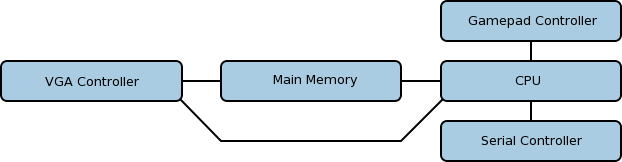
\includegraphics[width = 1\textwidth]{OverallOrganization.png}
	\caption{Overall Organization}
	\label{oo}
\end{figure}

A lot of the work required to render a game level to the screen is taken care of by hardware in the VGA Controller. There is a section in main memory where the map to be drawn is stored as a series of tile numbers, the VGA Controller reads these tile numbers from main memory, and for each tile number looks in its internal memory for the pixel map corresponding to the tile number and draws the pixels in the right section of the screen. The CPU has two registers which are directly wired to the VGA controller that tell the VGA controller where to look in main memory for the tile to be placed at the upper left corner of the screen and also what the row offset is. This makes the code for scrolling the screen to show only a section of the entire map as simple as setting the address for the upper left corner of the screen to a different location, rather than having the CPU rewrite the entire map area with new data to scroll.

\section{CPU Design}
Our CPU is composed of a control module, register file, ALU, instruction register, progam counter, processor status register, VGA start address register, VGA row length register, system clock module, a two input 16 bit multiplexor and a four input 16 bit multiplexor. (See figure \ref{cpu})

\begin{figure}[h!]
	\centering
	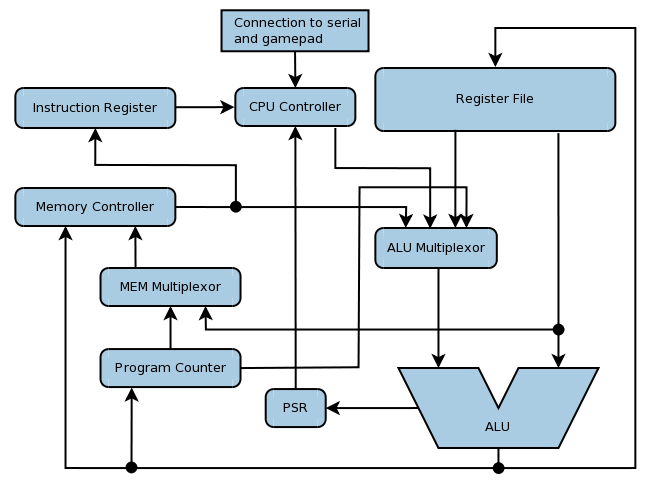
\includegraphics[width = 1\textwidth]{CPU_Diagram.png}
	\caption{CPU Design}
	\label{cpu}
\end{figure}

The CPU control module is a state machine with two states: fetch and execute. In the fetch state the memory address contained in the program counter is accessed and stored in the instruction register. In the execute state the control unit sets the control lines to all modules in order to execute the given instruction. The memory clock is inverted with respect to the CPU clock, and since the memory can be clocked at up to 800Mhz while our CPU is clocked at 25Mhz memory accesses are completed within a single CPU cycle.




\section{VGA Controller}
We used a 640$\times$480 VGA display with a 25 Mhz clock. This was done with the use of sync signals, and memory manipulation. The 640$\times$480 pixel display was broken up into 20$\times$15 blocks on the screen. This allowed us to conserve memory and still have meaningful graphics.  The graphics used 3 bit colors, and we were able to display 8 different colors. Using different patterns with these colors we were able to display 14 32$\times$32 pixel images.

\subsection{Sync Signals}
For the monitor to recognize which pixel it is on, it needs to receive 2 signals, Vsync and Hsync.  These signals will be sent on specific patterns because it generates different resolutions. We used a 25 Mhz clock input to generate the different signals. While we generated the signals, we kept track of which columns and rows the VGA was on. We used the columns and rows to find out which group of pixels it was on.  As well as the individual sub pixels that it is on in the 32$\times$32 block of pixels.

\subsection{VGA Memory}
We had organized our memory to have 2 separate memory blocks.  Main memory used a 2 port 14 bit addressable memory block containing 16 bit words. Our VGA memory contained a 14 bit addressable single port containing 9 bit words.  One of the 9 bit words contains 3 separate pixels.   We used each memory value twice, so we display the value of 3 bits for 2 pixels. We have an input to the bit generator where the starting address and row size of the image are.  This way we can fetch the entire cell in main memory that we would like to display.

\begin{figure}[h!]
	\centering
	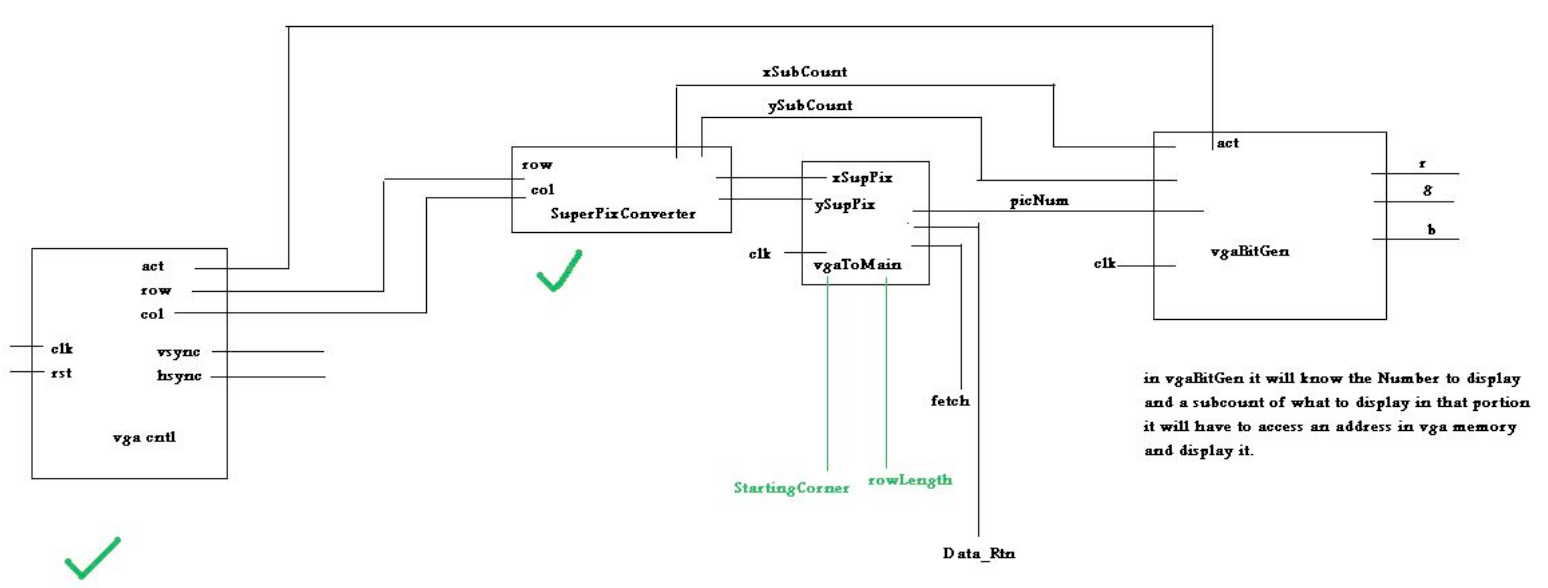
\includegraphics[width = 1\textwidth]{VGAdiagram.png}
	\caption{}
	\label{vga}
\end{figure}

In main memory we have an area specially set aside just for our levels.  These memory words contain a number from 0 to 14.  These words are related to the image that we want to display on that portion of the screen.  The VGA controller will read from main memory, find out what should be displayed on the block of the screen based on what number it is, and then go and display all of the values on the screen based on the number from 0 to 14.  From that number it will find the correct address in VGA memory that it should display for that pixel. 
 

\section{NES Controller}
For our game system we used a classic Nintendo Controller (figure \ref{nes}). This device required 5 lines to the controller: Power, Ground, Latch, Pulse, and Data.  The timing input for our controller was 25 Mhz, the module throttle was around 1Mhz and we achieved around 100 samples per second. This allowed us to read the input, detect whether the values were high or low and store it in a register. 

\begin{figure}[h!]
	\centering
	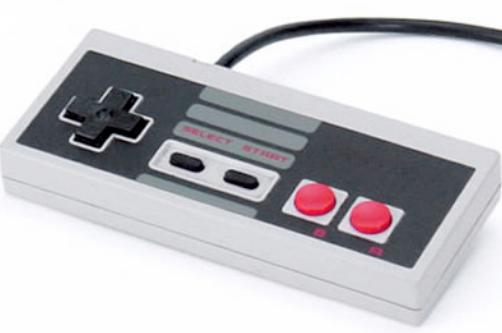
\includegraphics[width = .5\textwidth]{nescontroller.png}
	\caption{Classic Nintendo Gaming Controller}
	\label{nes}
\end{figure}

For us to read the data from the controller we had to generate two signals (Figure \ref{neswave}).  The Latch signal will be generated every time one wishes to read the Data signal. The Latch pulse width is 2 times the length of the Pulse signal�s pulse width. The Latch initiates the data read and the pulse intitiates each new chunk of data. While the Latch is high the Data line will provide the signal for the A button � 5V for pressed, and 0V for not pressed.  After the Latch signal is sent, the Pulse signal will need to send 7 pulses for the rest of the buttons. After that signal is sent, the data can pause until the controller sends the next Latch signal.  In our case

\begin{figure}[h!]
	\centering
	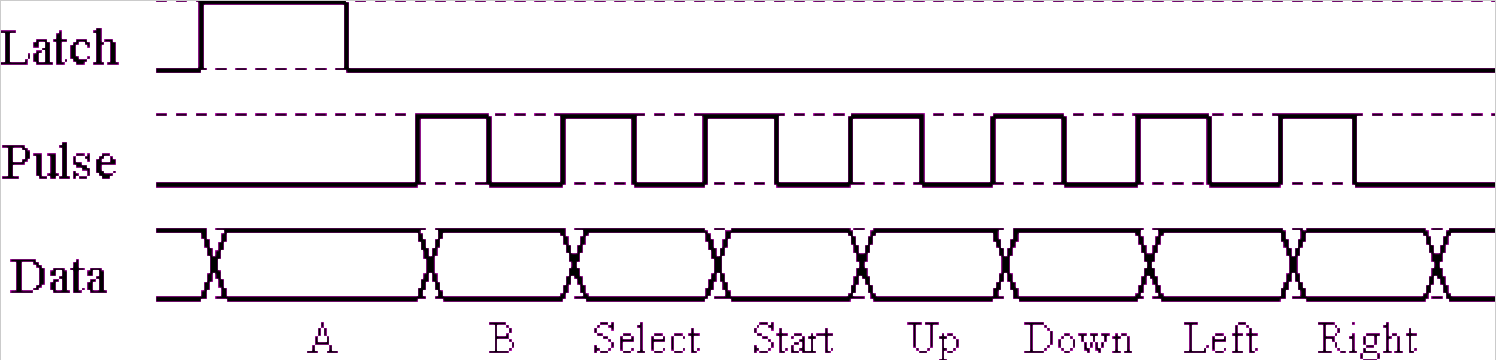
\includegraphics[width = 1\textwidth]{neswave.png}
	\caption{}
	\label{neswave}
\end{figure}

We were able to test if the controller would work with 3.3V logic versus the 5.0V logic that it states it needs.  We established that it is compatible with both logic levels, and that the Vt levels were probably around 2.5V.

\section{Serial Controller}

\section{Assembler}

\section{Software}

\section{System Integration}

\section{Conclusions and Further Work}

\section{Individual Contributions}

\subsection{Levi Balling}

\subsection{Robert Christensen}

\subsection{T. James Lewis}

\begin{thebibliography}{99}

\bibitem{Serial} Serial Interface (RS-232) \texttt{fpga4fun.com/SerialInterface.html}

\end{thebibliography}
\end{document}
